Design Space Modeling is the central part of the Design Flow Process of Cyber-Physical Systems (CPS). The Design Flow Process in AVM META is truly challenging involving many diverse interactions (designed and accidental) among components, in different physical domains (mechanical, thermal, electromagnetic, electrical, hydraulic, etc.) and across the interface between computational and physical. Interactions can be expressed as dependencies at design time or as physical power flows and information flows at run time. If designers and their design process are not prepared to recognize and manage such interactions, developments can suffer lengthy design iterations, and, at worst, failure due to unintended interactions discovered late in the design cycle, at integration time. For this reason, it is absolutely critical to correctly model the Design Space, including not only the plethora of design choices available, but also complex platform constraints to ensure that the chosen designs satisfy the requirements of the design. These design constraints arise not only from interactions among the individual components, but also due to functional and practical requirements of the design. For example, a bigger transmission works only if a diesel engine with large enough torque is used, or the vehicle must be able to acceleration a 2 m/s2 on a 20-degree uphill. Such constraints are complex to represent and require support for complex mathematical functions in the constraint language. The CyPyML Design Space Modeling provides a collection of modeling methods and tools for exploration and visualization of designs and design spaces, solving complex design constraints, and effective management of the design spaces and designs.

\subsubsection{Syntax}

\begin{figure}[t]
\centering
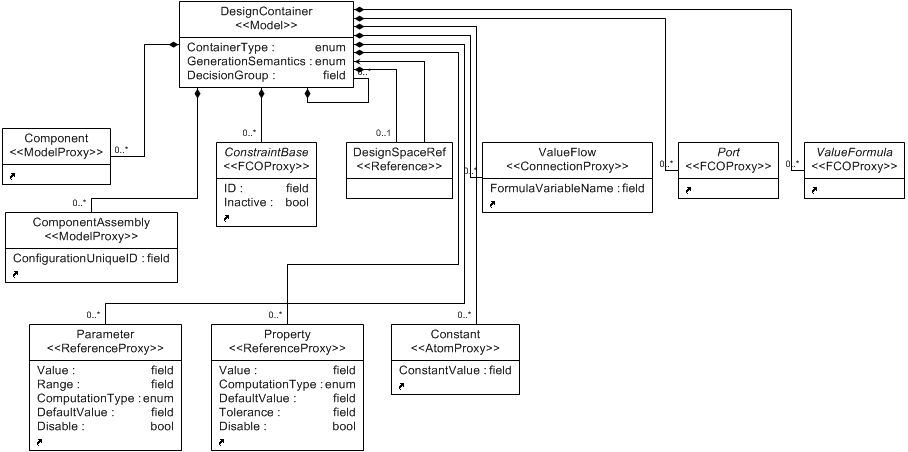
\includegraphics[scale=0.40]{Figures/DesignSpaceMetamodel.png}
\caption{Design Space Metamodel.}
\label{fig:designspacemetamodel}
\end{figure}

Figure \ref{fig:designspacemetamodel} shows the key modeling elements of CyPhyML pertaining to Design Space Modeling. As shown in the figure, the root element of the design space is of type DesignContainer. A DesignContainer can contain Components, Component Assemblies, Constraints, and DesignContainers. This allows to hierarchically model the Design Space mainly following the structural properties of the design. The enumeration shown for the DesignContainer's attribute ContainerType can have three possible values, viz. Compound, Alternative, or Optional. For a Compound DesignContainer, all its constituent elements must be selected as part of the design. Whereas, for an Alternative DesignContainer, only one among the choices available must be part of the design. The Optional DesignContainer contains only one DesignElement (a Component or a DesignContainer), which may or may not be part of the final design (i.e., optional containment).

\begin{figure}[t]
\centering
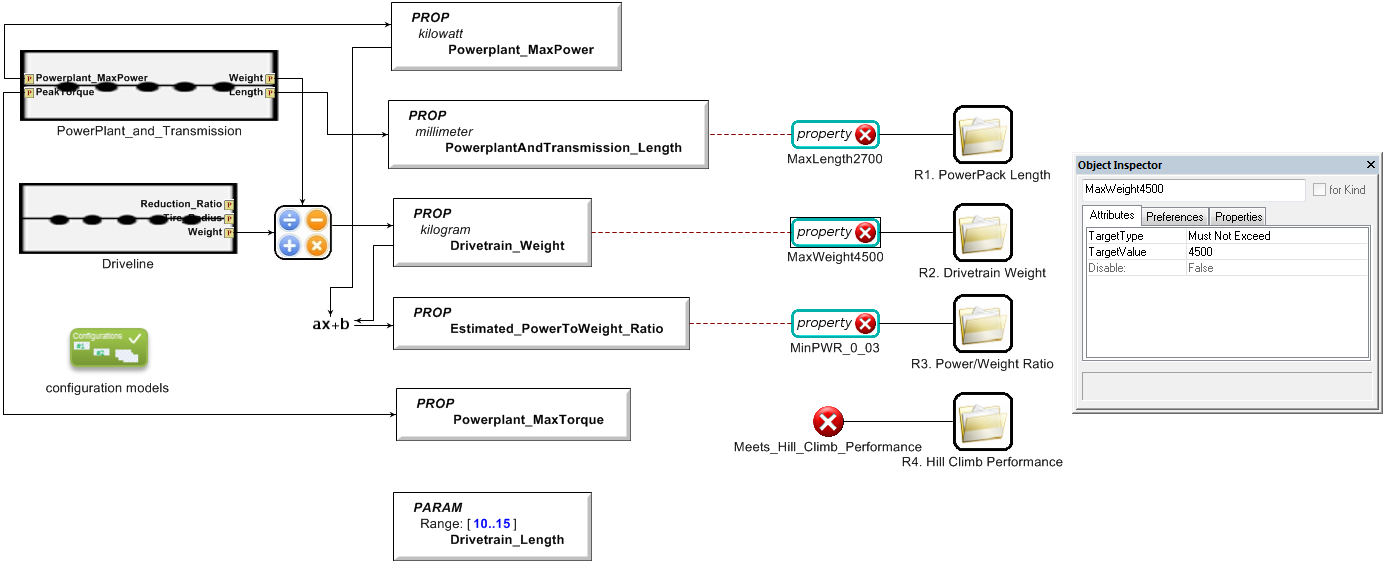
\includegraphics[scale=0.30]{Figures/IFVDrivetrainDesignSpace.png}
\caption{IFV Drivetrain Design Space Top-Level View.}
\label{fig:ifvdrivetraindesignspace}
\end{figure}

Figure \ref{fig:ifvdrivetraindesignspace} shows the top-level view of the IFV design space created using CyPhyML Design Space Modeling. The top-level design space itself is a Compound DesignContainer. In addition, it contains two child DesignContainers, viz. PowerPlant\_and\_Transmission and Driveline, both of which are Compound DesignContainers. The top-level DesignContainer also contains several design properties such as Powerplant\_MaxTorque and Drivetrain\_Weight. The properties of a DesignContainer may correspond to a basic property at that level in the DesignSpace or it may be a representative property that is calculated based on the chosen sub-elements of the DesignContainer. For example, the value of Drivetrain\_Weight property in a design will depend on which components were selected in that particular design. Design constraints can be applied on these properties. In addition to properties, CyPhyML also supports design parameters. Instead of taking a single value, design parameters can be used to specify a range of acceptable values for those parameters using the double-dot separator. The figure shows that the acceptable value of Drivetrain\_Length must be between 7-10 meters. The range can vary from -infinity to +infinity. Multiple ranges of parameters can be specified separated by a comma. These ranges specified for parameters are automatically translated into design constraints to ensure that the values of the parameters determined for acceptable designs are within acceptable ranges specified. Interested reader is referred to the secion on Property and Parameters for further information.

\begin{figure}[t]
\centering
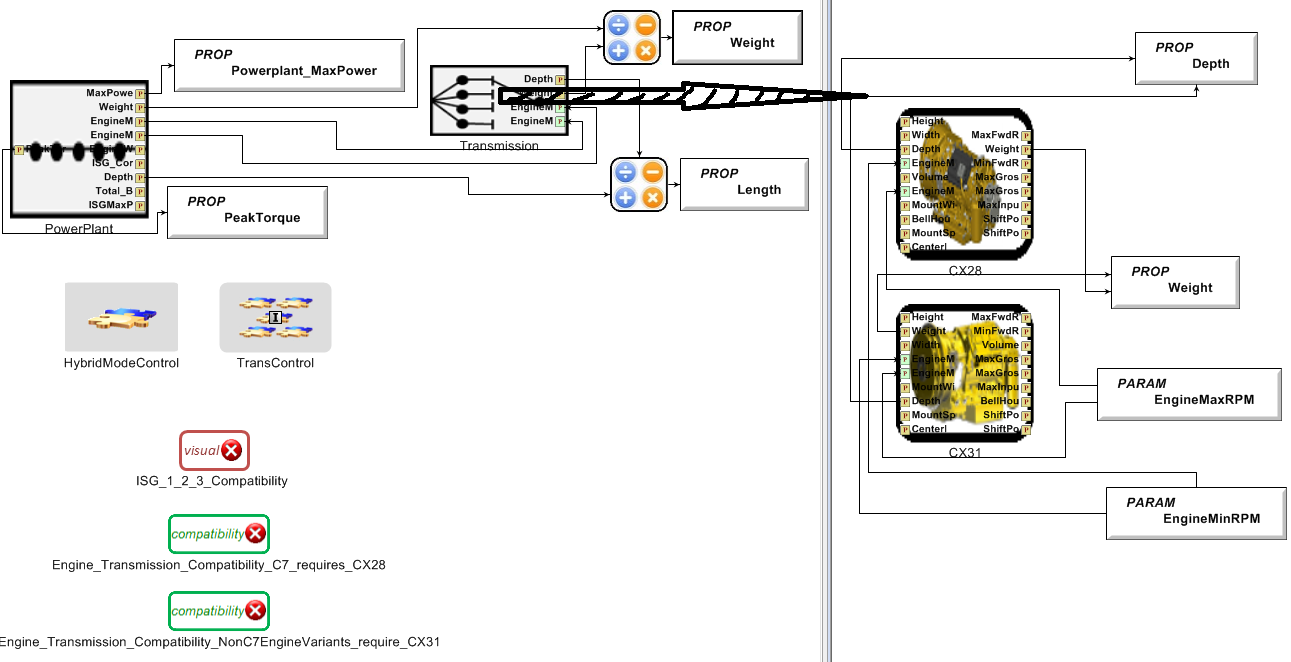
\includegraphics[scale=0.30]{Figures/AlternativeDesignContainer.png}
\caption{Alternative DesignContainer for Transmission and its Contents.}
\label{fig:alternativedesigncontainer}
\end{figure}


\paragraph{Alternative DesignContainers}

In the IFV drivetrain design space, the container PowerPlant\_and\_Transmission contains an Alternative DesignContainer for the transmission because two transmissions are available to choose for the design. Figure \ref{fig:alternativedesigncontainer} shows the Alternative DesignContainer for Transmission and shows its contents when expanded. As can be seen the IFV drivetrain has a choice of two transmissions, viz. CX28 and CX31.

\begin{figure}[t]
\centering
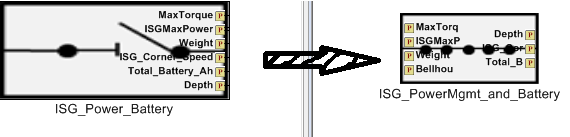
\includegraphics[scale=0.50]{Figures/OptionalDesignContainer.png}
\caption{ISG Power Battery Optional DesignContainer and its Contents.}
\label{fig:optionaldesigncontainer}
\end{figure}

\paragraph{Optional DesignContainers}

As show in Figure \ref{fig:optionaldesigncontainer}, in the IFV drivetrain design space, the container ISG\_Power\_Battery is an Optional DesignContainer. It contains only one DesignElement called ISG\_PowerMgmt\_and\_Battery. This means that in a IFV design ISG\_PowerMgmt\_and\_Battery may or may not be present (depending on whether the hybrid drivetrain control is used or not).

\paragraph{Constraints}
The feasible set of designs for a design space contains all possible combinations of the choices represented in the design space. This set contains an exponentially huge number of designs. However, not all designs are valid. To ensure that only meaningful and valid designs are selected, CyPhyML Design Space Modeling specification of several types of design and performance constraints. CyPhyML's DEsign Space ExploRaTion Tool (DESERT) ensures that only those designs are selected that satisfy the constraints modeled in the design space.

\subparagraph{PropertyConstraint}
Property constraints are the most basic type of constraints. It basically constrains the value of the associated property to be less than, less than or equal to, equal to, greater than or equal to, or greater than a specified value. In figure \ref{fig:ifvdrivetraindesignspace}, the property constraint is shown on IFV drivetrain maximum weight and ensures that the maximum drivetrain weight is less than or equal to 4500 Kgs.

\subparagraph{VisualConstraint}

\begin{figure}[t]
\centering
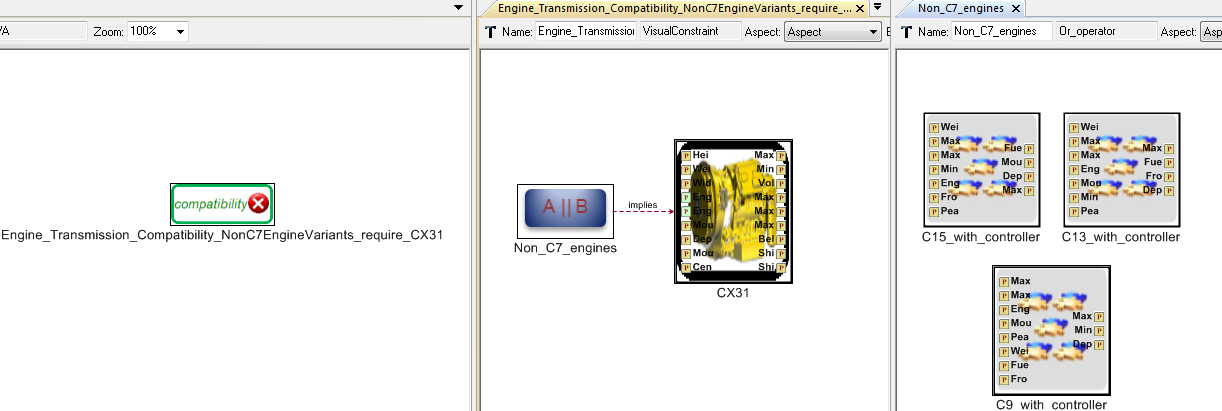
\includegraphics[scale=0.30]{Figures/DesignSpaceVisualConstraint.png}
\caption{Visual Constraint -- Engine\_Transmission\_Compatibility\_NonC7EngineVariants\_require\_CX31.}
\label{fig:designspacevisualconstraint}
\end{figure}

VisualConstrains are used to easily specify compatibility constraints in CyPhyML. In figure {fig:ifvdrivetraindesignspace}, several compatibility constraints are shown. One of them is Engine\_Transmission\_Compatibility\_NonC7EngineVariants\_require\_CX31. Figure \ref{fig:designspacevisualconstraint} shows the constraint fully expanded. Note that it uses an Or operator to combine variants of diesel engines that are not C7 and then uses an implies connection with the transmission CX31 to apply the compatibility constraint.

\begin{figure}[t]
\centering
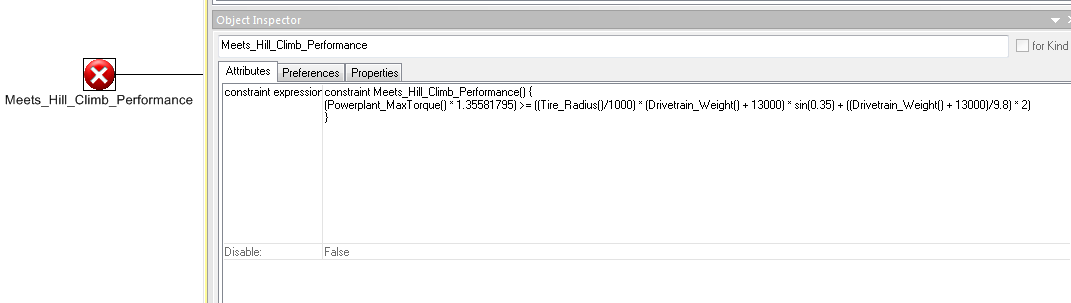
\includegraphics[scale=0.30]{Figures/DesignSpaceTextualOCLConstraint.png}
\caption{Example of manually written raw OCL-like CyPhyML design space constraint.}
\label{fig:designspacetextualoclconstraint}
\end{figure}

\subparagraph{Constraint Language}
All constraints in CyPhyML Design Space modeling are converted into raw OCL form. Although graphical means such as property constraints, parameter ranges, and visual constraints are sufficient to specify all types of constraints supported in CyPhyML, user can still choose to write them in textual OCL format, if needed. As an example, the constraint Meets\_Hill\_Climb\_Performance in figure \ref{fig:ifvdrivetraindesignspace} is a manually written constraint in raw OCL-like form. This is further shown in figure \ref{fig:designspacetextualoclconstraint}.

\subparagraph{DecisionGroup}

In the design space example above, the Driveline DesignContainer inside IFV drivetrain contains 8 HalfShaft\_and\_WheelAssembly DesignContainers. Each of these 8 DesignContainers are Altenative DesignContainers and contain choices of 3 different types of wheels. This leads to a total 3**8 = 6561 combinations just for choosing the wheels. However, in any IFV design, all wheels should be of same type. So, in reality there are only 3 choices. To represent that we can add several Visual constraints to make sure that if one type of wheel is chosen for any container, then same wheel type is chosen for all other 7 containers. However, this is highly cumbersome. CyPhyML provides an easier way to co-relate this same decisions of different Alternative DesignContainers by means of DecisionGroups. A DecisionGroup contains references of Alternative containers that essentially belong to the same decision of the choice that needs to be made. CyPhyML's DESERT solver recognizes DecisionGroups and automatically ensures that in any design same DesignElement is chosen for all Alternative DesignContainers that are part of the same DecisionGroup.

\subsubsection{Executing, Exporting, and Refinement}

Once the Design Space has been modeled along with all the compatibility, correctness, and performance constraints, the next step involves invoking the DESERT tool to generate configurations (point designs) that satisfy all the design space constraints. User is referred here to the DesignSpaceHelper tool document for further information (DesignSpaceHelper.docx). The configurations generated are lightweight such that they only contain references of the components chosen and no hierarchy or connections. These design can be converted into fully-specified designs with hierarchy and connections by using CyPhyML's tool called CyPhyCAExporter. User is referred to document CyPhyCAExporter\_OneSheet.docx for further information about it. One of the critical requirements of Design Space exploration and configuration generation is the capability to perform coarse-grained exploration and constraint satisfaction on some parts of the design space and when satisfactory configurations have been generated, do deeper refinement of those parts on the selected results. Such a capability is provided by CyPhy design refinement tool. User is referred to the document CyPhyDSRefiner..docx for further information on CyPhyML's design space refinemnet tool. CyPhyML also provides a tool called CyPhyDSEConverter. This tool allows the user to convert existing components, component assemblies, or design containers into a new design container that can now include new parts in it for design extentions and exploration of that particular child design space part of the original design space. User is referred to the document CyPhyDSEConverter.docx for more information on it. Lastly, CyPhyML also provides a tool to assist the user in determining the usefulness of refining a particular component, component assembly, or a design container. This tool is called CyPhyCriticalityMeter. CyPhyCriticalityMeter goes through all design spaces in the model and generates valid design configurations for them in memory and assigns a number to each DesignElement to specify how many configurations that DesignElement was chosen in and out of how many total configurations. User is referred to the document CyPhyCriticalityMeter.docx for more information on it.